\documentclass[12pt,letterpaper]{scrreprt}
\usepackage{subfigure}
\usepackage[latin1]{inputenc}
\usepackage{amsmath}
\usepackage{amsfonts}
\usepackage{amssymb}
\usepackage{graphicx}
\usepackage{todonotes}
\usepackage{appendix}
\usepackage{pdfpages}
\usepackage{lineno}
\usepackage{url}
\usepackage[colorlinks=true,linkcolor=blue,citecolor=blue,urlcolor=blue]{hyperref}

\linenumbers

\author{P. Bachant, M. Wosnik, B. Gunawan, V. Neary}
\title{Test Plan: UNH RM2 Tow Tank Experiment}

\begin{document}

\begin{titlepage}
    \centering
    \addtolength{\topmargin}{.5in}
    {\bfseries \large
        Experimental Test Plan: 1:6 Scale Reference Model 2 Cross-Flow Turbine
    }  
    \vskip1cm
    P. Bachant$^1$\\
    M. Wosnik$^1$\\
    B. Gunawan$^2$\\
    V. Neary$^2$\\  
    \vfill
    $^1$Center for Ocean Renewable Energy \\
    University of New Hampshire \\
    Durham, NH \\
    \vspace{0.1in}
    $^2$Water Power Technologies \\
    Sandia National Laboratories \\
    Albuquerque, NM \\
    \vfill
    November 7, 2014
    \vfill
    \textbf{Prepared by:}\\
    Center for Ocean Renewable Energy\\
    University of New Hampshire\\
    Durham, NH\\
    \vspace{0.1in}
    \textbf{Prepared for:} \\
    Wind and Water Power Technologies Program \\
    Office of Energy Efficiency and Renewable Energy \\
    U.S. Department of Energy \\
    Washington, D.C.
    \vfill
    
\includegraphics[width=0.32\textwidth]{Figures/unhlogo} \\
    \vspace{0.1in}
    
\includegraphics[width=0.41\textwidth]{Figures/snllogo} \\
    \vspace{0.1in}
    
\includegraphics[width=0.34\textwidth]{Figures/doelogo}
    \vfill
\end{titlepage}

\tableofcontents

\chapter{Introduction}

The blades of cross-flow turbines experience large variations in angles of
attack as they rotate about their axis (``cross-flow turbine'' means the axis of
rotation is perpendicular to flow direction---can be vertical or horizontal).
This range of angles of attack becomes larger as the tip speed ratio
$\lambda=\omega R/U_\infty$ decreases \cite{Para2002}. The variation is
typically sufficiently large that the blades operate under dynamic stall, which
is a complex unsteady process, deviating significantly from static foil
behavior. Furthermore, the higher the solidity of a cross-flow turbine, the
lower the optimal tip-speed ratio at which it operates. Marine Hydrokinetic
(MHK) cross-flow turbines typically have higher solidity than cross-flow wind
turbines (VAWT), and hence operate at lower tip-speed ratios. Since MHK turbines
operate in a higher density fluid, unsteady dynamic effects related to the
blades' pitching motion and flow curvature also become more important when
compared to wind turbines.

The performance of cross-flow MHK turbines thus depends on both Reynolds number
and solidity (note that these issues are related, since an average blade chord
Reynolds number, $Re_{c,\mathrm{avg}} \approx \lambda U_\infty c/ \nu$, can be
expressed in terms of tip speed ratio, which is a function of solidity). If
numerical models are validated with physical model data that was obtained at
insufficiently high Reynolds numbers, it cannot be determined whether problems
with model predictions are caused by Reynolds number effects, issues related to
higher solidity, or both. It is uncertain whether numerical models validated
with physical model data obtained at low Reynolds number should be considered
validated at all, since the scale at which the model will be applied is orders
of magnitude larger. One way to overcome this uncertainty is to show that the
scaled physical model test has become Reynolds number independent, and therefore
validation efforts should be relevant at full-scale. 

For example, the effect of Reynolds number on average power output was shown to
be significant on the 2 m Sandia Research Darrieus turbine in wind tunnel
testing \cite{Blackwell1976}: Maximum power coefficient, $C_{P,\mathrm{max}}$,
increased with Reynolds number, $Re_c$, along with a shift of the location of
$C_{P,\mathrm{max}}$ toward lower tip speed ratios due to delayed blade stall.
The effects of Reynolds number were quite dramatic over a relatively small range
of $Re_c \approx 1.1 \times 10^5$--$2.9 \times 10^5$. More recently, Bachant and
Wosnik \cite{Bachant2014} showed that turbine performance and near-wake
characteristics become Reynolds number independent at $Re_c \approx 2 \times
10^5$.

To date, attempts to validate the CACTUS model have relied on measurements from
the Saint Anthony Falls Laboratory (SAFL) \cite{Hill2014} and the University of
New Hampshire (UNH) \cite{Neary2013, Michelen2014}. For the SAFL experiments
(RM2), the chord Reynolds number, $Re_c \sim 10^4$, was below the threshold
needed to properly simulate lift and stall characteristics. For the UNH
experiment \cite{Bachant2013}, the chord Reynolds number was sufficiently high
at $Re_c \approx 2.7 \times 10^5$, but the chord/radius ratio and solidity
(13.4\%) created instability in the free-wake evolution, which caused
significant overestimation of power coefficient.

The present task is therefore to acquire a new dataset for the lower solidity
RM2 turbine, but at higher Reynolds numbers. It is also suspected that the strut
drag model in CACTUS may be causing some discrepancy, so providing some hard
data for comparison will help sort out that question. This dataset will be
publicly available for both validation of CACTUS and other numerical models.


\section{Study goals, objectives, and milestones}

The overarching goal of this project is to collect a Reynolds number independent
performance dataset for a 1:6 scale RM2 turbine, which is repeatable, and which
can be used to investigate the accuracy of numerical models, e.g., mid-fidelity
models such as CACTUS. These mid-fidelity models are needed by MHK developers to
predict the performance of their cross-flow turbine designs, since physical
modeling at appropriate scales can be prohibitively expensive in the early
stages of engineering. Furthermore, Navier--Stokes-based computational fluid
dynamics (CFD) simulations require modeling in 3 dimensions, which generally
necessitates high performance computing---a resource that is not commonly
available, and more expensive.

The project will provide insight on the physics of hydrokinetic cross-flow
turbines, including the importance of blade strut drag on turbine power output,
which will determine what level of focus is necessary in improving mid-fidelity
modeling of these effects. The experimental dataset will be shared publicly and
can be used for validating other numerical models/codes used by developers and
DOE partners. The study goals can be distilled into the following main
objectives:

\begin{enumerate}

	\item Acquire a Reynolds number independent dataset for the DOE RM2 cross-flow
	turbine. This task involves the following subtasks:

		\begin{enumerate}
			\item Design and build an appropriate turbine model.
		
			\item Acquire full device performance curves (power and drag coefficients) at
			multiple $Re$, to attempt to find convergence.
		  
			\item Once convergence is found, acquire another performance curve at that
			Reynolds number $Re_0$.
		
			\item If time permits, acquire a detailed wake flow map in the near-wake at
			$Re_0$ using acoustic Doppler velocimetry.
		\end{enumerate}
	
	\item Measure the effects of strut drag on RM2 performance. This objective will
	require that we:
	
	\begin{enumerate}
		\item Measure the parasitic torque from support struts by rotating the turbine
		in still water. \label{obj-parasitic_torque}
		
		\item Redo task \ref{obj-parasitic_torque} with cylindrical tubes slid over
		the struts to significantly increase drag.
		
		\item Acquire a performance curve at $Re_0$ with the high-drag struts. 
	\end{enumerate}
	
\end{enumerate}

\section{Milestones}
The progress of this project will be marked by the completion of the following:

\begin{enumerate}

	\item \textbf{November 7, 2014} -- Experimental test plan draft and turbine
	model design reviewed.
	
	\item \textbf{January 16, 2015} -- Turbine model assembled.
	
	\item \textbf{March 30, 2015} -- Experimental data collected, processed, and
	basic report written.

\end{enumerate}


\chapter{Experimental setup and methods}

\section{Turbine model}

The turbine is to be a 1:6 scale model of the DOE RM2 rotor, reproduced as
faithfully as possible. Turbine geometry is to be scaled from the RM2 ``rev 0''
design report \cite{Barone2011}, with the exception of the shaft diameter, which
will be a scaled version of the SAFL RM2 shaft \cite{Hill2014}. The hub design
is also similar to the SAFL model, which may aid in comparison of the results,
though this is not a top priority. Geometric parameters are shown in
Table~\ref{tab-turb_geom} and a drawing of the turbine design is shown in
Figure~\ref{fig-turbine_drawing}. See Appendix~\ref{app-turbine_dwgs} for
manufacturing drawings.

\begin{table}[ht]
\centering
\begin{tabular}{l|l|l}
   & Full-scale & Model (1:6) \\
\hline 
Diameter (m)   & 6.450 & 1.075 \\ 
Height (m)     & 4.840 & 0.8067 \\ 
Blade root chord (m) & 0.4000 & 0.06667 \\ 
Blade tip chord (m)  & 0.2400 & 0.04000 \\ 
Blade profile & NACA 0021 & NACA 0021 \\ 
Blade mount & 1/2 chord & 1/2 chord \\ 
Blade pitch (deg.) & 0.0 & 0.0 \\ 
Strut profile & NACA 0021 & NACA 0021 \\ 
Strut chord (m) & 0.3600 & 0.06000 \\ 
Shaft diameter (m) & 0.2540 \cite{Beam2011} or 0.4160 \cite{Hill2014} & 0.06350\\ 
\end{tabular}
\caption{RM2 turbine geometric parameters.}
\label{tab-turb_geom}
\end{table}

\begin{figure}[ht]
\centering
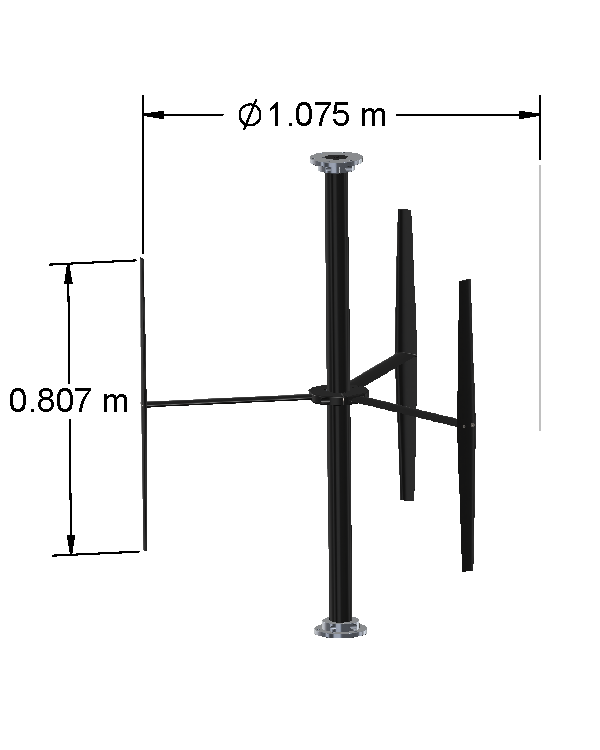
\includegraphics[width=0.5\textwidth]{Figures/turbine}
\caption{Illustration of the UNH RM2 scaled physical model.}
\label{fig-turbine_drawing}
\end{figure}


\section{Facility and instrumentation}

Experiments will be performed in the UNH tow/wave tank, a 36 m long facility
with a 3.66 m wide by 2.44 m deep cross-section. The turbine will be mounted in
a frame built from NACA 0020 struts, attached to the tow carriage by four linear
bearings, which transfer all streamwise force to a pair of S-beam load cells.
The turbine shaft RPM will be controlled by a servo motor system, which allows
prescription of the turbine tip speed ratio. The load torque will be measured by
an inline rotary torque transducer and a load cell mounted at a fixed distance
from the servo motor, providing a redundant measurement. Turbine shaft angle
will be measured using the servo drive's emulated encoder output, set to $10^5$
counts per turbine shaft revolution. Carriage speed, and therefore inflow
velocity will be measured using a linear encoder with 10 $\mu$m resolution.
Turbine wake measurements at 1 turbine diameter downstream will be measured with
a Nortek Vectrino+ acoustic Doppler velocimeter, sampling at 200 Hz. A list of
the sensors to be used in the experiment is shown in Table~\ref{tab-sensors},
instrumentation in Table~\ref{tab-instrumentation}, and a drawing of the
experimental setup is shown in Figure~\ref{fig-exp_setup}.

\begin{table}[ht]
\centering
\begin{tabular}{c|c|c|c}
Measured quantity & Device type & Mfg. \& model & Accuracy \\
\hline 
Carriage position & Linear encoder & Renishaw LM15 & 10 $\mu$m/pulse \\
Turbine angle & Drive encoder output & Kollmorgen AKD & 10$^5$ pulse/rev \\
Turbine torque & Rotary transducer & Interface T8-200 & $\pm$0.5 Nm \\ 
Turbine torque (2) & Load cell (\& arm) & Sentran ZB3-200 & $\pm$0.2 Nm \\
Drag force, left & Load cell & Sentran ZB3-500 & $\pm$0.6 N \\
Drag force, right & Load cell & Sentran ZB3-500 & $\pm$0.6 N \\
Fluid velocity & ADV & Nortek Vectrino+ & $\pm$0.5\% val. $\pm$1 mm/s \\
\end{tabular}
\caption{Details of the sensors to be used for the experiment. Note that ``(2)''
denotes a secondary redundant measurement.} 
\label{tab-sensors}
\end{table}

\begin{table}[ht]
\centering
\begin{tabular}{c|c|c|c}
Measured quantity & Device type & Mfg. \& model \\
\hline 
Carriage position & Differential counter & NI 9411 \\
Carriage velocity (2) & Motion controller & ACS NTM \\
Turbine angle & Differential counter & NI 9411 \\
Turbine RPM (2) & Motion controller & ACS NTM \\
Turbine torque & Analog voltage input & NI 9405 \\ 
Turbine torque (2) & Analog bridge input & NI 9237 \\
Drag force, left & Analog bridge input & NI 9237 \\
Drag force, right & Analog bridge input & NI 9237 \\
\end{tabular}
\caption{Details of the instrumentation to be used for the experiment. Note that
``(2)'' denotes a secondary redundant measurement.}
\label{tab-instrumentation}
\end{table}

\begin{figure}[ht]
\centering
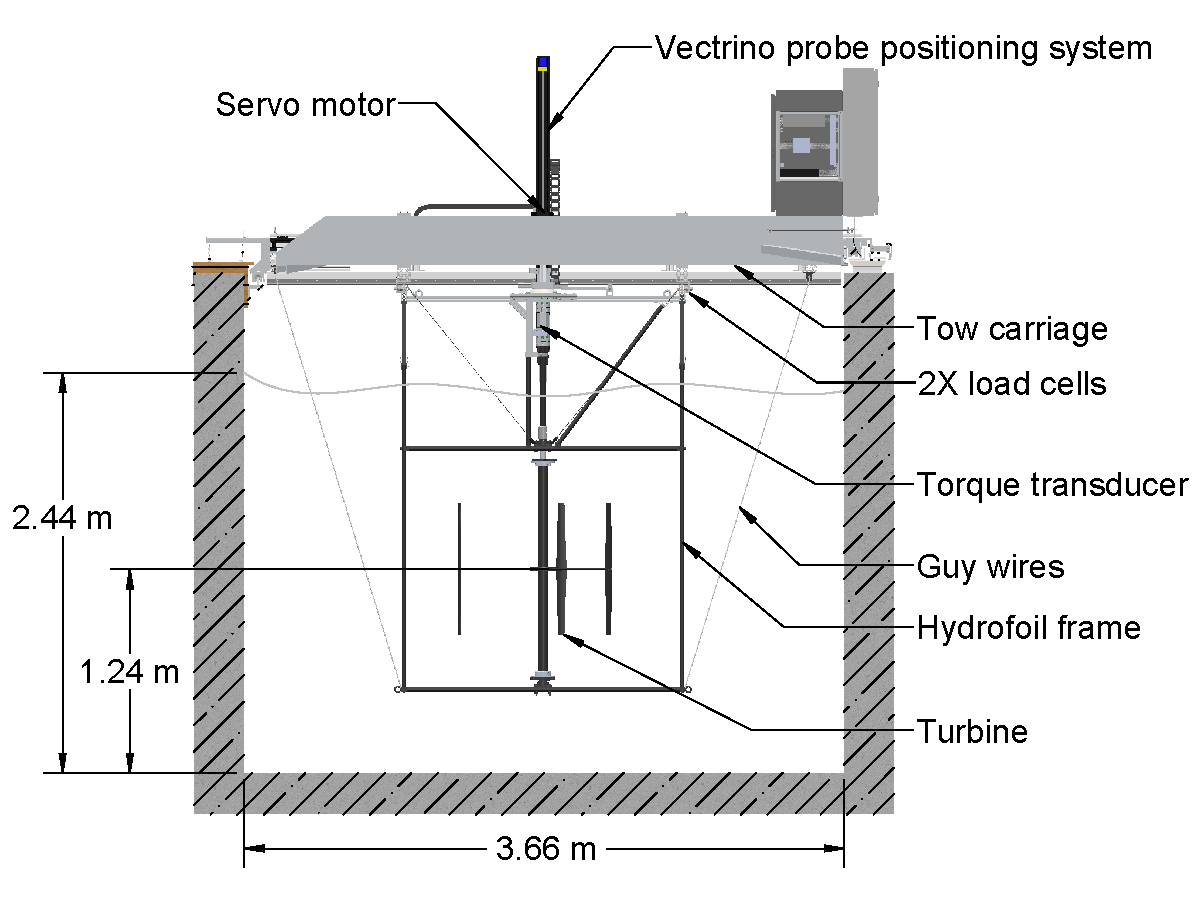
\includegraphics[clip,trim=0.01in 0 0 0, width=\textwidth]{Figures/tank_cross_section}
\caption{Illustration of the experimental setup.}
\label{fig-exp_setup}
\end{figure}


\chapter{Research deliverables}

A full performance curve for the turbine will consist of 20--30 tows at varying
tip speed ratio. Each of these tows will produce raw data for the turbine
torque, drag force on the submerged equipment, turbine shaft angle, carriage
speed, and Vectrino velocity measurements. Raw data files will be saved from our
data acquisition device at a sample sate of 2 kHz, from the motion controller at
1 kHz, and from the Vectrino at 200 Hz. All three devices will be triggered by
the motion controller at the beginning of each run so that they are relatively
synchronized.

Tare torque and drag runs will also be performed to measure the shaft bearing
friction torque and turbine mounting frame drag, respectively. These data will
be similar to the turbine performance data, omitting torque measurements for the
tare drag runs and vice versa.

Raw data will be stored in HDF5 format, run metadata in text-based JavaScript
Object Notation (JSON), processed data in comma separated value (CSV), and
processing code in Python. Raw data files will be uploaded to
figshare\footnote{\url{http://figshare.com}}, which will then give the dataset a
Digital Object Identifier (DOI) and therefore a persistent URL. Processed data
and processing code will be hosted on GitHub\footnote{\url{https://github.com}}
to help facilitate updates to the analysis by both the investigators and third
parties. This processing code will be written such that raw data is downloaded
automatically as needed. Versions  or ``releases'' of the Git repository will be
uploaded to figshare such that they will have their own DOIs, and can be cited
appropriately in publications. Lastly, a report detailing the experiment and the
results will be written and included as part of the repository. All research
products---documentation, data, code, CAD models, etc.---will be freely
available under a Creative Commons Attribution 4.0 International license, which
allows further sharing and adaptation so long as the original source is
credited.

\renewcommand{\bibname}{References}
\bibliography{../Resources/Library}
\bibliographystyle{abbrv}

\begin{appendices}

\chapter{Turbine model manufacturing drawings}

\label{app-turbine_dwgs}

\includepdf[pages={1-3}, landscape]{../Drawings/Assembly-RM2-UNH.pdf}
\includepdf[pages={1}, landscape]{../Drawings/Blade.pdf}
\includepdf[pages={1}, landscape]{../Drawings/Strut.pdf}
\includepdf[pages={1}, landscape]{../Drawings/Shaft.pdf}
\includepdf[pages={1}, landscape]{../Drawings/Hub-section.pdf}
\includepdf[pages={1}, landscape]{../Drawings/Plug-shaft-locating.pdf}
\includepdf[pages={1}, landscape]{../Drawings/Spacer-blade-mount.pdf}
\includepdf[pages={1}, landscape]{../Drawings/Strut-cover.pdf}
\includepdf[pages={1}, landscape]{../Drawings/Insert-strut-cover.pdf}
\includepdf[pages={1}, landscape]{../Drawings/End-cap-strut-cover.pdf}

\end{appendices}

\end{document}